\chapter{Theory}\
This chapter introduces the necessary theoretical background to
understand the work done in this thesis.

%\begin{figure}[]
%    \centering
%    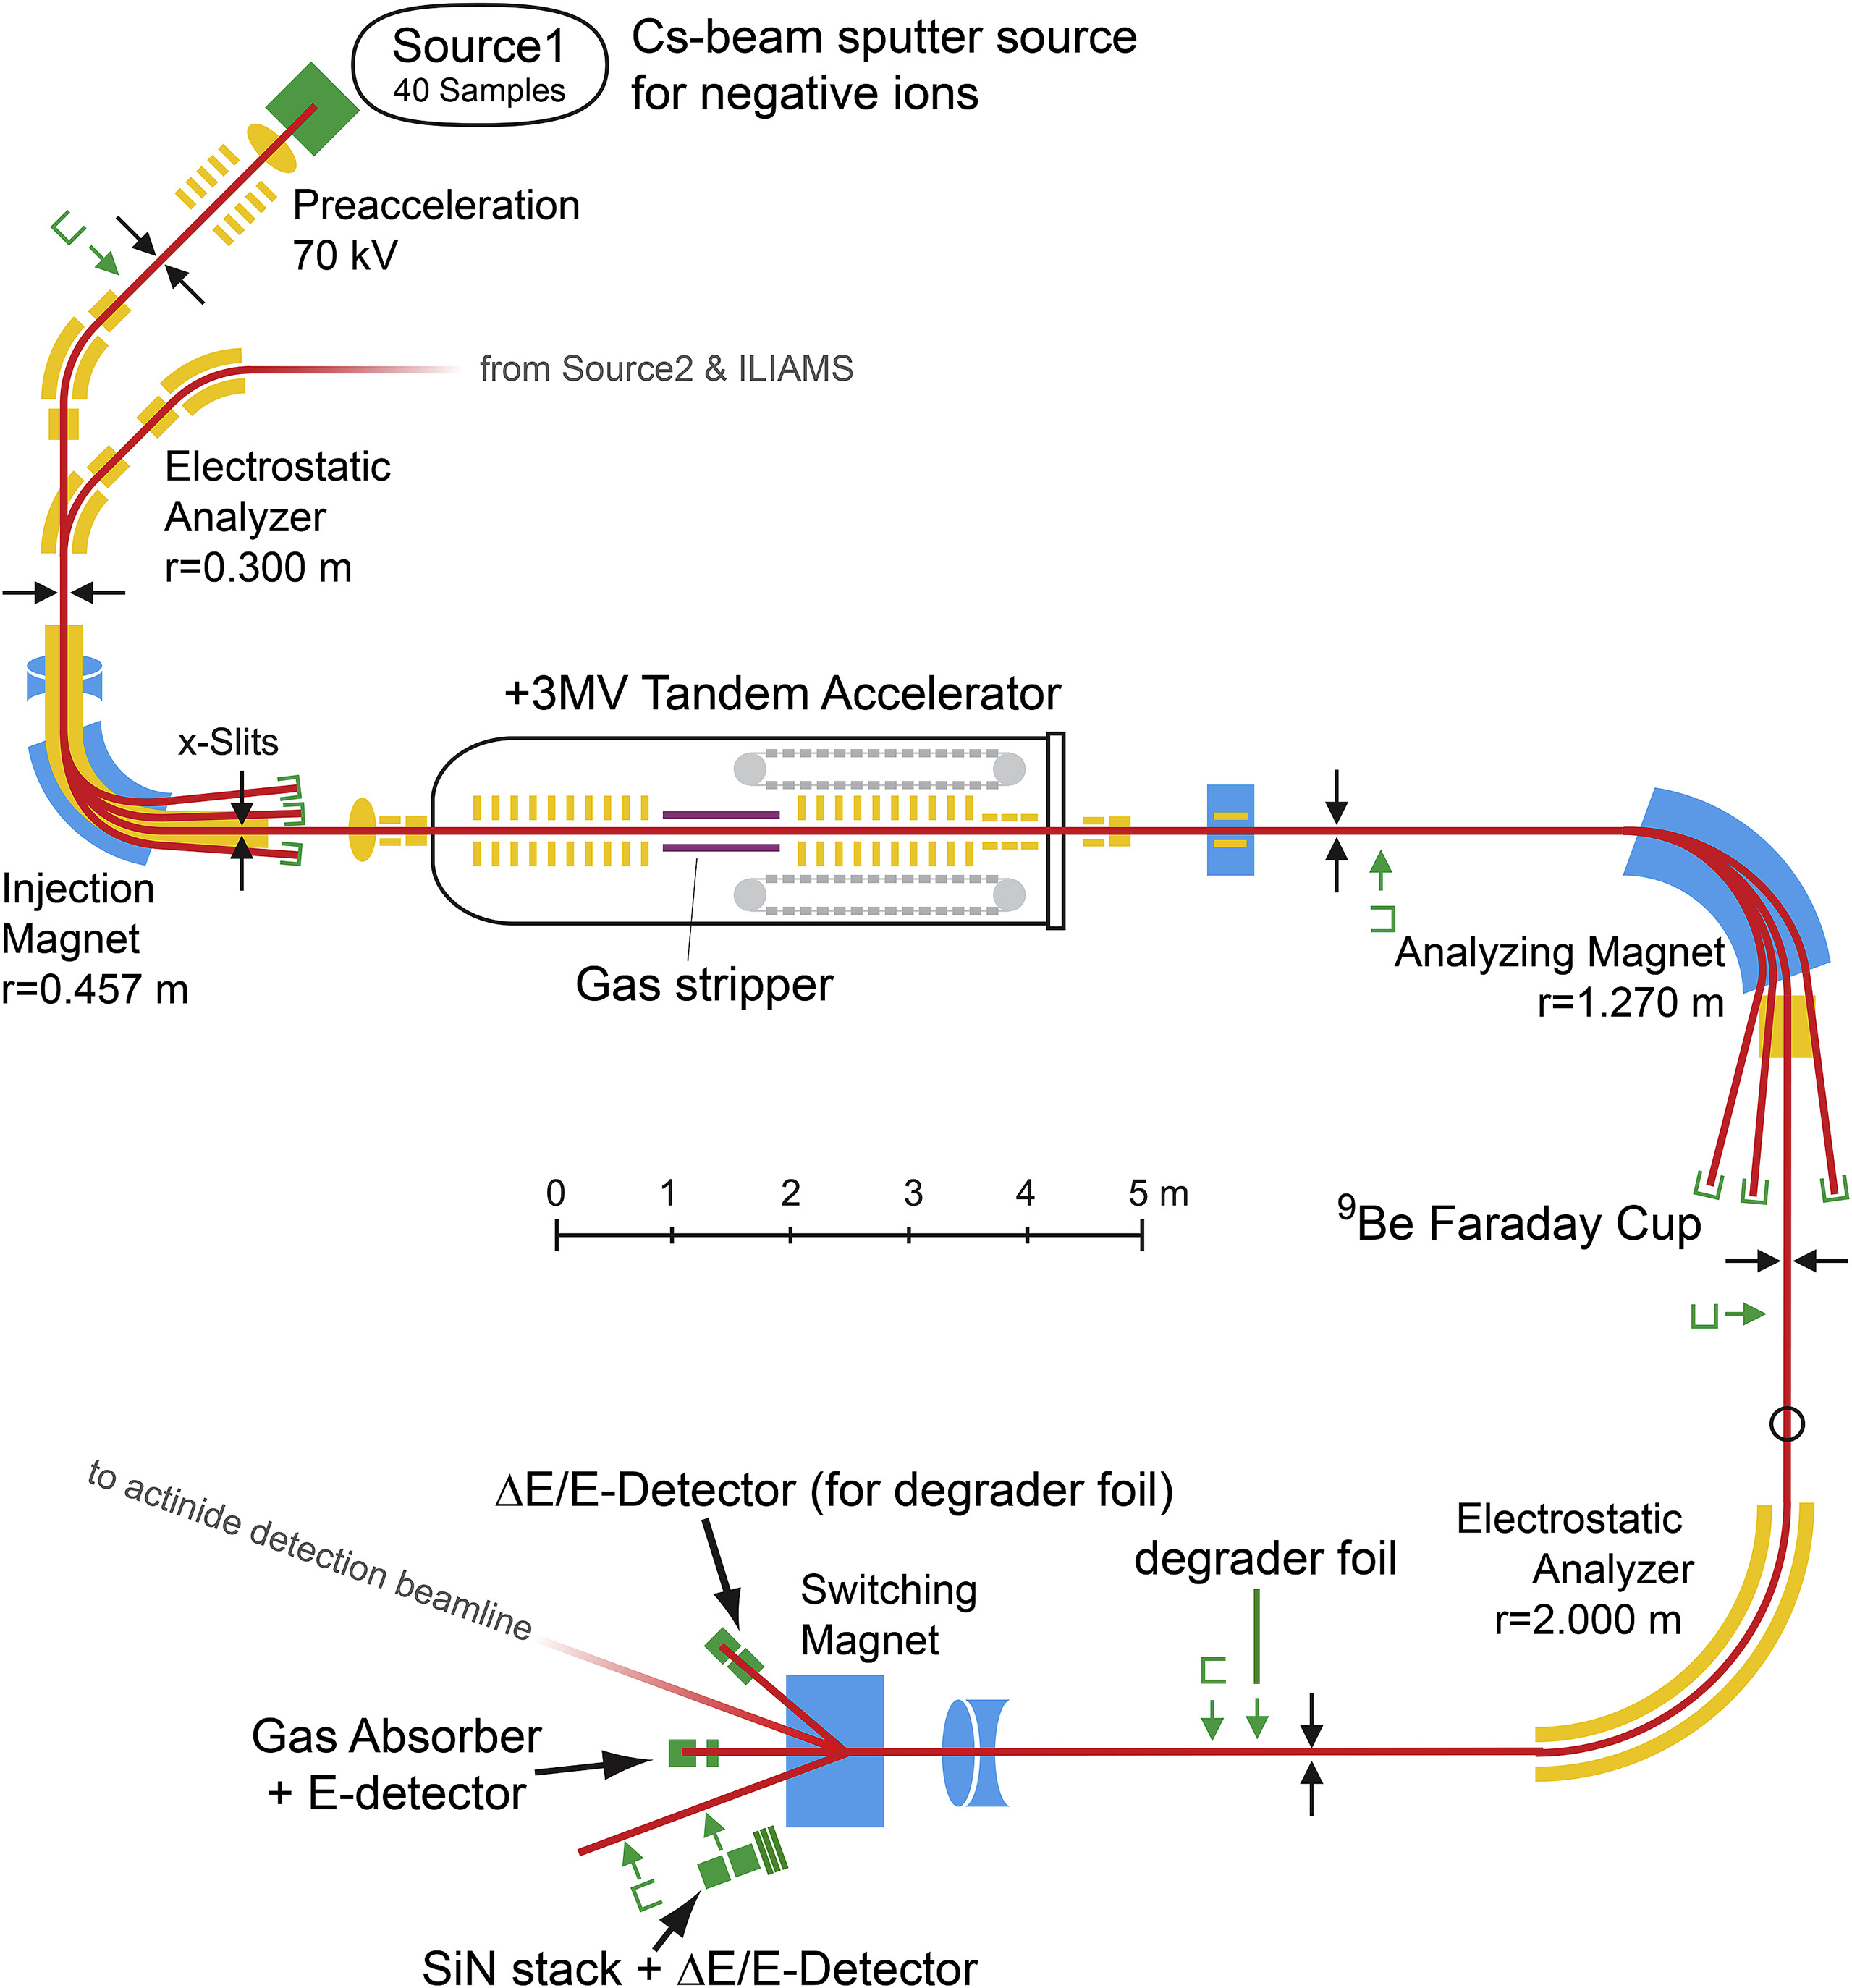
\includegraphics[width=\textwidth]{B/Steier2019_BeStackedFoilMethod_AMS_drawing.jpg}
%    \caption{Schematic layout of the VERA facility used for \ce{^{10}Be} from Ref.\cite{steier2019}.}
%    \label{fig:enter-label}
%\end{figure}


\section{Principles of AMS}
This section is based on Refs.\cite{schuur2013radiocarbon} and  \cite{tuniz1998ams}. The general equipment layout for AMS and the process is illustrated on \cref{fig:AMS} and this section will explain the theoretical knowledge needed to understand the fundamental processes in AMS.
\begin{figure}[ht]
    \centering
    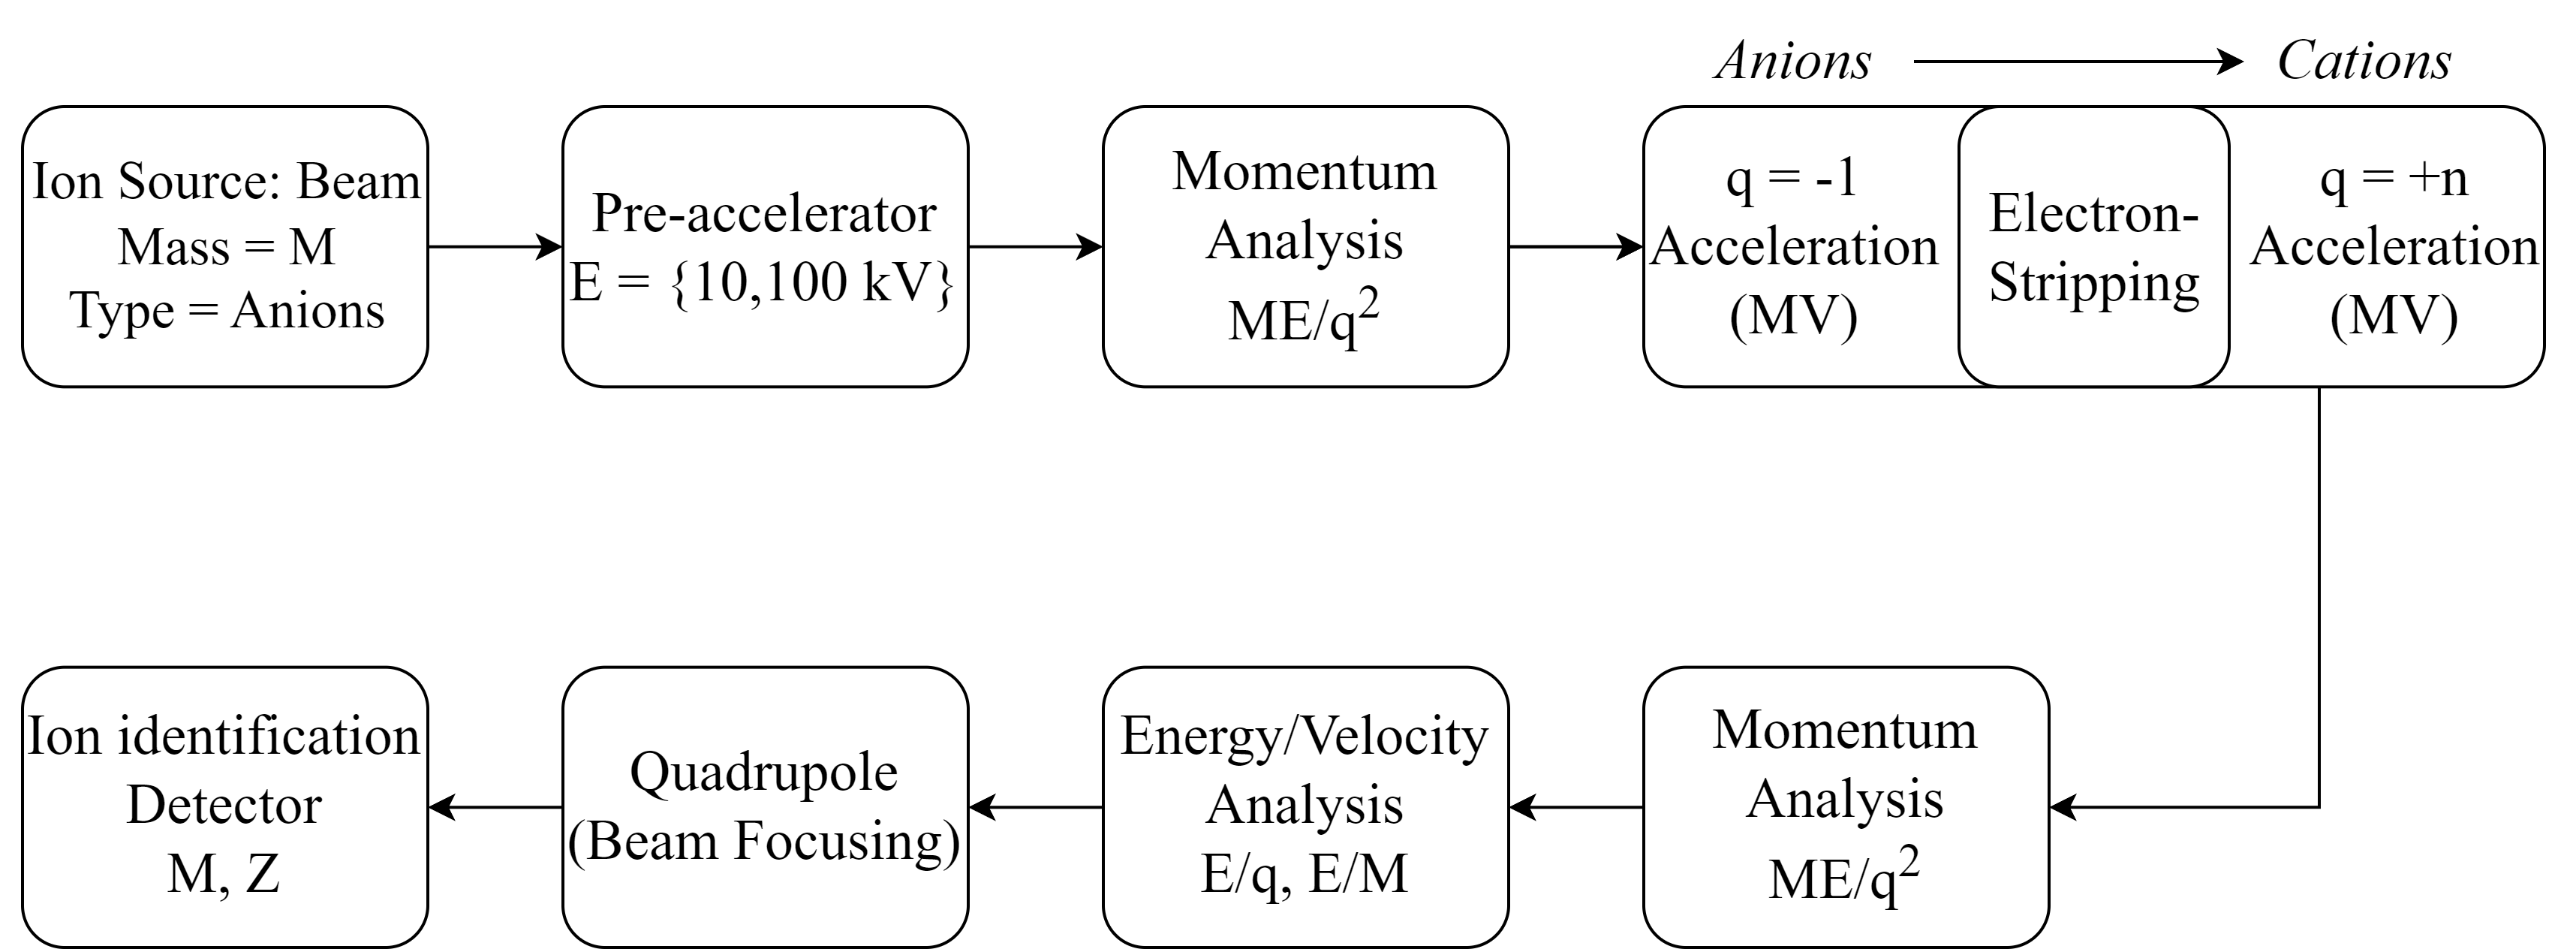
\includegraphics[width=\textwidth]{B/AMS.png}
    \caption{Schematic layout of equipment for AMS based on Ref.\cite{tuniz1998ams}.}
    \label{fig:AMS}
\end{figure}

\subsection{Ion Sputter Source}
An AMS sputter source typically consists of a system with a heated \ce{Cs} reservoir, where \ce{Cs} vapor is maintained at a pressure of approximately $10^{-4}$ mbar. This vapor is pumped into a cavity (see \cref{fig: Sputter ion source}). The cavity, which includes the ionizer, is constructed from a metal with a low work function, such as tantalum, tungsten, or molybdenum. The low work function refers to the energy required to remove an electron from the metal's interior to a point just outside its surface. This area is heated to 1000 Celsius to thermally ionize the \ce{Cs} into \ce{Cs^{+}} (Cations). The symmetry of the cavity is constructed so that the \ce{Cs^{+}}-ions are focused to hit the sample target - with
their newly gained energy by applying an electric potential between the ionizer and the sample target - and ejecting atoms from its surface.

The applied voltage will dictate whether it's negative (Anions) or positive (Cations) ions we want to extract and further accelerate away from the ion source. The energy of the ions emitted is

\begin{equation}
    E_{source} =  eq (U_{ex}+U_{tar})
\end{equation}
where $e$ is the elementary charge and $q$ is the charged state \cite{schuur2013radiocarbon}.

\begin{figure}[ht]
    \centering
    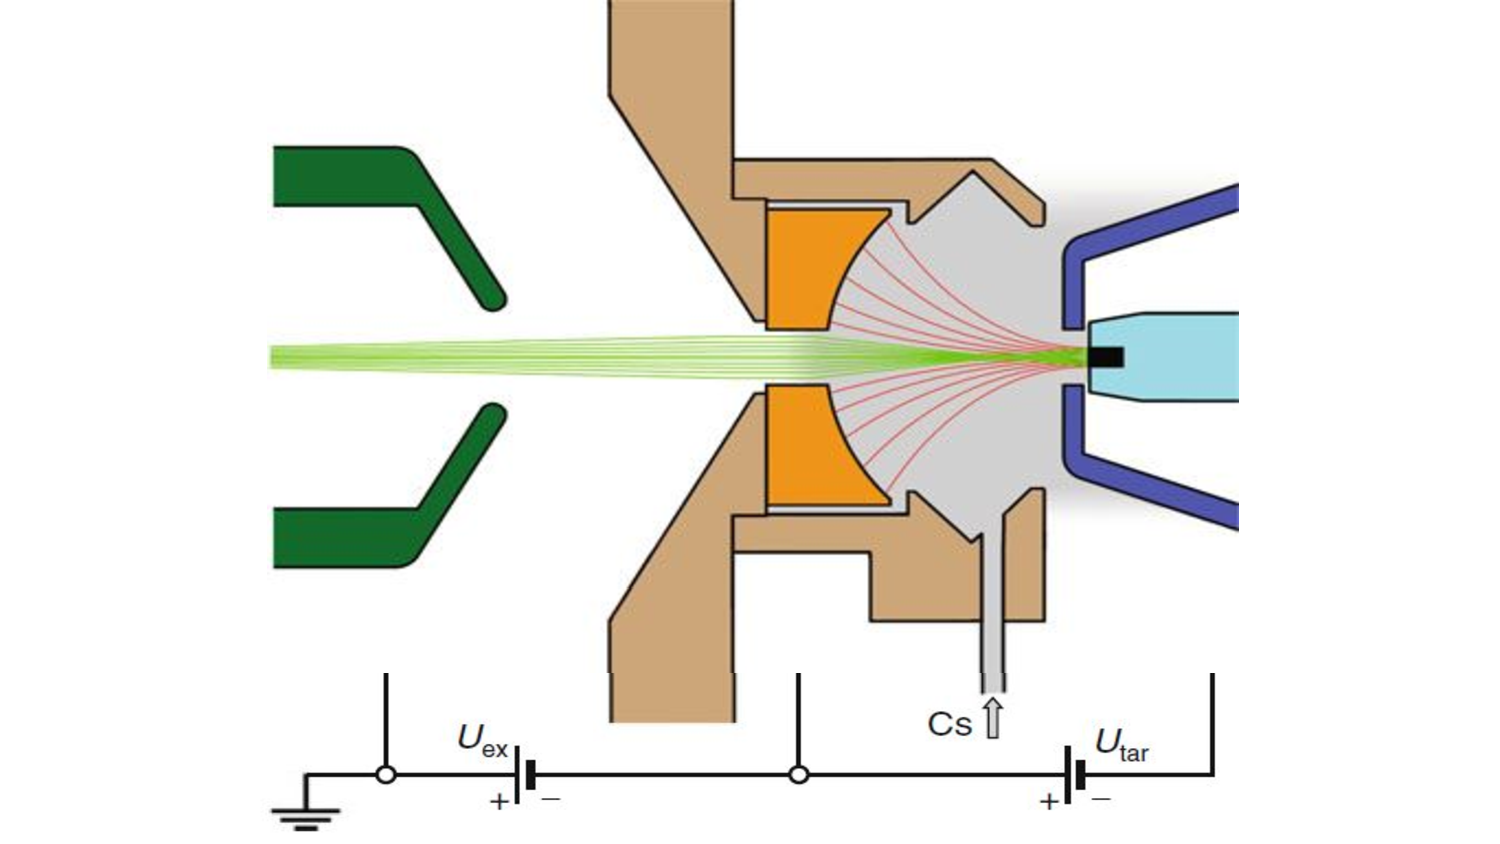
\includegraphics[width=1\columnwidth]{B/Generalized schematic of a sputter ion source.pdf}
    \caption{A generalized schematic of an ion sputter source for generating negative ions. Cs vapor is produced and introduced into the ion source via a tube (gray arrow). On the heated surfaces of the ionizer (orange), Cs atoms are ionized (red lines), which are focused onto the sample (black) within the metal target (cyan) by the target voltage ($U_{tar}$). As the \ce{Cs^{+}} ions sputter the target, negative carbon ions, \ce{Cs^{-}}, (light green) are generated and then accelerated by $U_{tar}$, followed by the extraction voltage ($U_{ex}$).}
    \label{fig: Sputter ion source}
\end{figure}

\subsection{Magnets}\label{Magnetssection}
The beamline of \ce{Ce^{-}} has a charge of $q = -1$, and therefore, a field is needed if they are to be moved along the AMS setup. 
Commonly known as a bending/injection (BI) magnet used for moment analysis, it is used to steer the beamline of \ce{Cs^{-}} into the correct path, particularly as it enters or is injected into the accelerator.\\

When a charged particle moves perpendicular to a magnetic field, it experiences a magnetic force that causes it to move in a circular trajectory. The force due to the magnetic field provides the centripetal force necessary for this circular motion. By equating the centripetal force with that of the Lorentz force equation, $F = qvB$, and utilizing the kinetic energy and velocity of the charged particle - $E_{kin}=E_{source}=\frac{1}{2}Mv$ and $v=\sqrt{\frac{2E_{kin}}{M}}$ respectively. For an ion, $X(q,p)$, with charge $q$ and momentum $p = \sqrt{2\cdot A \cdot E}$ in a homogenous magnetic field, $B$ the radius, $r$, of the curvature of its trajectory can be determined by analyzing these relationships yielding
\begin{equation}
    \left(\dfrac{M}{q}\right)\left(\dfrac{E_{kin}}{q}\right)=k_{1}(Br)^{2}
    \label{magnetrigitidy}
\end{equation}\\

An energy/velocity analyzer is often placed post-acceleration of the beamline and is also known as an ESA. ESA is an instrument that uses electric fields to separate charged
particles (ions) based on their energy per charge. The force on a charged particle in an electrostatic field 
\begin{equation}
    F = q  \mathcal{E}
\end{equation}
can be used with the work-energy theorem to determine the trajectory of the curvature imposed by the electrostatic field
\begin{equation}
    \dfrac{E}{q} = k_{2}\mathcal{E}r.
    \label{electricrigitidy}
\end{equation}

The charged ions' Lorenz force will cause the beamline to start spreading. Quadrupoles are utilized to gather the beamline.



\subsection{Tandem-Accelerator}
A tandem accelerator utilizes a two-stage acceleration process, which involves converting negative ions into positive ions. The device accelerates ions through an electric potential difference, which is achieved by creating a high-voltage terminal at the midpoint of the accelerator. This allows for efficient acceleration of particles to higher energies.

In the first stage, negative ions are injected into the accelerator with an initial energy $E_i = V_i e$, where $V_i$ is the injection voltage and $e$ is the electronic charge. As the negative ions are accelerated towards the high-voltage terminal, they pass through an electron stripper. The electron stripper removes electrons from the negative ions, converting them into positive ions with charge $q$, typically resulting in a higher charge state.

After passing through the electron stripper, the now positive ions are further accelerated by the terminal's high-voltage potential $V_{t}$. This results in an increase in the kinetic energy of the ions.

The total energy $E_f$ of the ions after acceleration is given by:
\begin{equation}
    E_f = E_i + (q + 1)eV_t
    \label{ionenergyafteracc}
\end{equation}
This equation shows that the final energy depends on the ions' initial energy and the terminal voltage.

For a more generalized expression of the ion energy $E$ after acceleration in the tandem, we can use:
\begin{equation}
    E = \left( \frac{(V_i + V_t) M_p}{M_i} + q V_t \right) e
    \label{higenergysection}
\end{equation}
Where $V_{i} e$ is the initial energy of the injected ions, $V_{t}$ is the terminal voltage, $e$ is the electronic charge, $q$ is the charge state of the ions after stripping, $M_p$ is the mass of the positive ion, and $M_{i}$ is the mass of the negative ion.

%This should be added to methodology???
%If the negative ion injected is a molecular ion that dissociates at the stripper, the mass of the resulting positive ion, $M_{p}$, will differ from the mass of the negative ion, $M_{i}$. If no dissociation occurs, the masses are equal.

\section{Isosbar}

\section{Cosmogenic Nuclide Dating}
\subsection{Nuclear reactions}
\subsection{Nuclear Decay}

\section{Stopping Power}